\section{Formulation of the problem}
\label{Formulation}
%==========================

\indent The primary goal is to deliver a payload, such as an egg to some height unharmed using a robot that is bio-inspired. The problem is broken up into two parts. The first part is to find a way to rapidly ascend updward.\\

%===================== Trajectory ==========
\begin{figure}[H]
\begin{center}
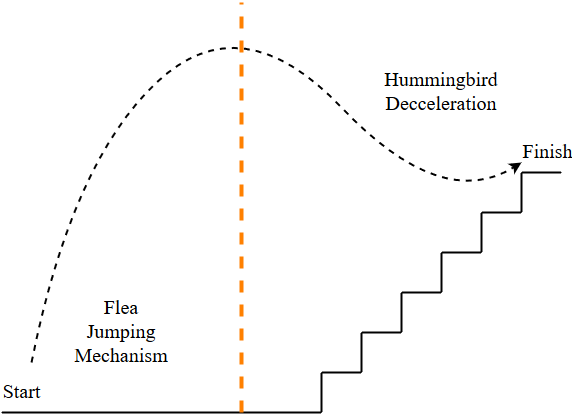
\includegraphics[width=0.75\linewidth]{./Figures/trajectory.png}
\caption{This is a visual representation of the goal of delivering an egg to the top of a staircase. The orange line separates the two different mechanisms into their respective roles for the trajectory of the payload.}
\label{fig:trajectory}
\end{center}
\end{figure}
%===================== Trajectory ==========

\subsection{Acceleration Mechanism}
\indent As shown in \textbf{Figure} \ref{fig:trajectory}, a jumping mechanism will be used to achieve substantial height for the payload delivery. In order to draw inspiration from how a flea uses its energy to jump so high, energy usage will be explored in relation to payload mass as well as maximum height. A flea can jump many times its own height, but it is small in mass, approximately 45mg \cite[p.~63]{bennet-clark_jump_nodate}. Fleas have a ratio of mass to jump height and energy density. For a larger robot, a similar ratio could be achieved if energy density is proportionally higher to account for the larger mass. The larger mass is in part introduced by the need to carry an egg, which a flea does not have.\\
%===================== Cap Free-Body Diagram ==========
\begin{figure}[H]
\begin{center}
\includegraphics[width=0.5\linewidth]{./Figures/capFreeBodyDiagram.png}
\caption{Simple three component flea system.}
\label{fig:capFreeBodyDiagram}
\end{center}
\end{figure}
%===================== Cap Free-Body Diagram ==========
\subsubsection{Dynamic Model}
\indent For simplicity, it is assumed that the femur and tibia have negligable mass. The vertical take-off mechanism is treated as a two-link planar robot leg.\\
% %===================== Kinematics Model ==========
% \begin{figure}[H]
% \begin{center}
% \includegraphics[width=0.5\linewidth]{./Figures/kinematics.png}
% \caption{Model for a planar, two-link, robot leg.}
% \label{fig:kinemaitcs}
% \end{center}
% \end{figure}
% %===================== Kinematics Model ==========
\noindent \textbf{Forward Kinematics:}
\begin{align}
    x = x_2 = \alpha_1\cos\theta_\text{hip} + \alpha\cos(\theta_\text{hip} + \theta_\text{knee})\\
    y = y_2 = \alpha_1\sin\theta_\text{hip} + \alpha\sin(\theta_\text{hip} + \theta_\text{knee})
\end{align}
\begin{equation}
    \begin{bmatrix}
        h_1(\theta_\text{hip},\theta_\text{knee})\\
        h_2(\theta_\text{hip},\theta_\text{knee})
    \end{bmatrix}
    =
    \begin{bmatrix}
        \alpha_1\cos\theta_\text{hip} + \alpha\cos(\theta_\text{hip} + \theta_\text{knee})\\
        \alpha_1\sin\theta_\text{hip} + \alpha\sin(\theta_\text{hip} + \theta_\text{knee})
    \end{bmatrix}
\end{equation}
\noindent This yields the following Jacobian:
\begin{equation}
    J =
    \begin{bmatrix}
        \frac{\partial h_1}{\partial \theta_1} & \frac{\partial h_1}{\partial \theta_2}\\
        \frac{\partial h_2}{\partial \theta_1} & \frac{\partial h_1}{\partial \theta_2}
    \end{bmatrix}
    =
    \begin{bmatrix}
        -l_\text{femur}\sin(\theta_\text{hip}) - l_\text{tibia}\sin(\theta_\text{hip} +\theta_\text{knee}) & -l_\text{tibia}\sin(\theta_\text{hip} +\theta_\text{knee})\\
        l_\text{femur}\cos(\theta_\text{hip}) + l_\text{tibia}\cos(\theta_\text{hip} +\theta_\text{knee}) & l_\text{tibia}\cos(\theta_\text{hip} +\theta_\text{knee})
    \end{bmatrix}
\end{equation}
\noindent From the resulting Jacobian the following relation is used:
\begin{equation}\label{jac}
    F_\text{end} = J^\text{T}F_\text{desired}
\end{equation}
\noindent where 
\begin{equation}
    F_\text{desired} = 
    \begin{bmatrix}
        f_{\dot{\theta}_{hip}}\\
        f_{\dot{\theta}_{knee}}
    \end{bmatrix}
\end{equation}
\noindent The components of $F_\text{desired}$ represent the forces due to torque associated with the knee and hip joints. Equation \ref{jac} shows the output force of the system provided with an input of desired torques, \cite{spong_robot_nodate}.
\noindent The resulting \textbf{orientation matrix} is as follows:
\begin{equation}
    \begin{bmatrix}
        x_2x_0 & y_2x_0\\
        x_2y_0 & y_2y_0\\
    \end{bmatrix}
    = 
    \begin{bmatrix}
        \cos(\theta_1 + \theta_2) & -\sin(\theta_1 + \theta_2)\\
        \sin(\theta_1 + \theta_2) & \cos(\theta_1 + \theta_2)\\
    \end{bmatrix}
\end{equation}
\textbf{Inverse Kinematics:}
\begin{align}
    \theta_1 & = \tan^{-1}\bigg(\frac{y_{des}}{x_{des}}\bigg)-\tan^{-1}\bigg(\frac{\alpha_1\sin\theta_2}{\alpha_1+\alpha_2\cos\theta_2}\bigg)\\
    \theta_2 &= \cos^{-1}\bigg(\frac{x_{des}^2 + y_{des}^2 - \alpha_1^2 - \alpha_2^2}{2\alpha_1\alpha_2}\bigg)
\end{align}
\indent The inverse kinematics represents the angles, $\theta_1, \theta_2$ of the two-link leg to be functions of a desired position, ($x_{des}, y_{des}$). When controlling the acceleration of the robot's mass upwards, the inverse kinematics will be used to command a position of the end of the robot leg at various time steps. A desired acceleration can be incorporated into a feedback loop, which is discussed further in \textbf{section} \ref{Control}. From the kinematics the following state-space model is derived:\\
\begin{equation}
    \bf{\dot{x}} = \bf{f}(\bf{x,u}) = 
    \begin{bmatrix}
        
    \end{bmatrix}
\end{equation}


\subsubsection{Control}